%%%%%%%%%%%%%%%%%%%%%%%%%%%%%%%%%%%%%%%%%
% University/School Laboratory Report
% LaTeX Template
% Version 3.1 (25/3/14)
%
% License:
% CC BY-NC-SA 3.0 (http://creativecommons.org/licenses/by-nc-sa/3.0/)
%
%%%%%%%%%%%%%%%%%%%%%%%%%%%%%%%%%%%%%%%%%

%----------------------------------------------------------------------------------------
%	PACKAGES AND DOCUMENT CONFIGURATIONS
%----------------------------------------------------------------------------------------

\documentclass[10pt]{article}
\usepackage[version=3]{mhchem} % Package for chemical equation typesetting \ce{}
\usepackage{siunitx} % Provides the \SI{}{} and \si{}
\usepackage{graphicx} % Required for the inclusion of images
\usepackage{natbib} % Required to change bibliography style to APA
\usepackage{amsmath} % Required for some math elements 
\usepackage{hyperref}
\usepackage{url}
\usepackage{color}
\usepackage{bm}
\usepackage{cancel}
\usepackage{float}
\restylefloat{table}
\setlength\parindent{0pt} % Removes all indentation from paragraphs

\renewcommand{\labelenumi}{\alph{enumi}.} % Make numbering in the enumerate environment by letter rather than number (e.g. section 6)

%\usepackage{times} % Uncomment to use the Times New Roman font

%----------------------------------------------------------------------------------------
%	DOCUMENT INFORMATION
%----------------------------------------------------------------------------------------

\title{The Development of a Peak Fitting and Finding Software for Gamma Spectroscopy Applications \\
\bigskip \large Final Project} % subtitle

\author{William \textsc{Gurecky}} % Author name

\date{\today} % Date for the report

\begin{document}

\maketitle % Insert the title, author and date

\begin{center}
\begin{tabular}{l r}
Date Performed: & May 1, 2017 \\ % Date the experiment was performed
Partners: &  N/A \\ % Partner names
&  \\
Instructor: & Dr.  Derek Haas % Instructor/supervisor
\end{tabular}
\end{center}
\tableofcontents

% If you wish to include an abstract, uncomment the lines below
%\begin{abstract}
%\end{abstract}

%----------------------------------------------------------------------------------------
%	SECTION 1
%----------------------------------------------------------------------------------------

\pagebreak
\section*{Definitions}
\label{definitions}
\begin{description}

\item[CWT]  Continuous wavelet transform.
\item[GUI]  Graphical user interface.
\item[NLS]  Non linear least squares.
\item[ROI]  Region of interest.

\end{description}

%----------------------------------------------------------------------------------------
%	SECTION 2
%----------------------------------------------------------------------------------------
\section{Introduction}
In this work an open source tool to perform peak finding, fitting and visualization is developed.  These tasks
are commonplace in the post processing of gamma ray spectroscopy data.
To this end, there are many available solutions.  The software
package Cambio produced by Sandia National laboratory is one such example.  The vast majority
of gamma ray peak post processing software is closed source and by nature is not easily extensible.
Additionally, the current work addresses some shortcomings present in some of the traditional
software, namely, the inability to deconvolve multiple nearby peaks and the lack of reliable automatic
peak detection.  As a result of the current work, a software packaged entitled GammaSpy was developed in python.
GammaSpy is freely available for download at: \url{https://github.com/wgurecky/GammaSpy}.  Though
this software solution does not represent a truly novel solution to the aforementioned issues, it does
provide a platform for students to easily analyze gamma spectra collected in the lab, and furthermore
is easily modified and extended if additional features are desired.

\section{Overview}

GammaSpy utilizes non-linear curve fitting techniques found in the open
literature and are freely available in open source python libraries.  To
decompose nearby peaks, an iterative solution based on basin hopping is used
which is a cousin of simulated annealing.  The automatic peak detection
algorithm used in GammaSpy is based on the continuous wavelet transform rather
than a derivative based approach to alleviate false negatives encountered when
one attempts to find peaks passed on the smoothed derivatives of the original
signal.  A discussion of how the software functions and how the user interacts
with the GUI are provided in this document. \\

The end user will interact with the underlaying numerical routines through a
graphical user interface. The GUI allows the user to navigate the spectrum, add
peaks, select ROI, fit peaks, and visualize the fitting results.
See section \ref{ug} for a brief introduction to the GUI.

\subsection{File Compatibility}
GammaSpy can read a variety of file formats commonly used in other gamma spectroscopy softwares.
\begin{itemize}
    \item Canberra *.CNF
    \item Canberra *.MCA
    \item Rigaku *.DAT
    \item Siemens *.UXD
    \item *.csv
    \item *.HDF5
\end{itemize}
This is essential for interoperability with data collection systems like Gini
or Maestro.  The ability to read myriad data formats is provided by the
excellent xylib python library available here: \url{xylib.sourceforge.net}. \\

It is possible to save spectra and fitting results to the HDF5 format.  HDF5 is
ideal for large data array storage as it supports on the fly compression of
many data types thus saving storage space.  Additionally, HDF5 files can be
read by many other plotting softwares and do not require a gamma spectroscopy
software to open. \\

An option to export fitted peak information to ASCII is also provided so that
the user can optionally write a parser or simply copy/paste the peak fitting
results into Excel. \\

\section{Methods}

\subsection{Peak Fitting}

In the current implementation all peaks are assumed to be Gaussian or a linear
combination of Gaussian distributions, however it is possible to substitute
more complex peak models in the future if required.  The local peak background
is modeled as linear.  When fitting a single peak, both the Gaussian parameters
and linear parameters are estimated simultaneously.  This gives rise to a
nonlinear least squares (NLS) problem assuming the Gaussian parameters are
allowed to vary.  Some constraints can be placed on the Gaussian parameters
such that only positive mean and height are allowed, however these constraints
do not guarantee that the NLS problem will be free of local minima.

In GammaSpy the NLS regression is cast as a chi-squared optimization problem.
The goal is to minimize the chi-squared objective function shown in equation \ref{err}:

\begin{equation}
    \chi^2 = \sum_i \frac{(y_i - \hat y_i)^2}{\sigma_{y_i}^2}
    \label{err}
\end{equation}
Where $\hat y_i$ are predicted values from the target function $y(x_i|\alpha_1,
.. \alpha_n)$ which has free model parameters $\bm{\alpha} = \{\alpha_1, ... \alpha_n\}$.
The squared differences are inversely weighted by the variance of each data
sample.  This effectively upweights the importance of counts with low variance
relative to counts with large variance.  In the case of a gamma spectrum the
variance of each bin is equal to it's height: $\sigma_{y_i}^2 = y_i$. \\

To minimize equation \ref{err}, newton's method is employed to find a local
minimum of the objective function.  To find a minimum to equation (\ref{err}), the partial derivatives of $\chi^2$ are
computed with respect to each free model parameter:
\begin{equation}
    E'(\bm \alpha) = \frac{\partial \chi^2}{\partial \{\alpha_1, ... \alpha_n\}} = 0
\end{equation}

With the $j^{th}$ iteration of newton's method given by:
\begin{equation}
    \bm \alpha^{j+1} = \bm \alpha^j -  \omega \frac{E'(\bm \alpha^j)}{ E''(\bm \alpha^j)}
\end{equation}
Where $E'$ is the Jacobian and $E''$ is the Hessian of the objective function with
respect to the free parameters, $\bm{\alpha}$.  The partial derivatives are estimated using
central finite differences as is implemented in the numdifftools python library (\url{https://pypi.python.org/pypi/Numdifftools}). $\omega$ is a successive over
relaxation parameter that helps damp oscillations about the minimum when set $<1.$, and is
typically set to 0.9 in GammaSpy.  Newtons method is terminated when:
\begin{equation}
    \left\lVert \frac{\bm \alpha^j - \bm \alpha^{j+1}}{\bm \alpha^j}\right\rVert < tol
\end{equation}
And the relative tolerance is selected to be $\SI{1e-6}$.

This however, does not guarantee convergence
to the global minimum in the case of NLS.  Instead, GammaSpy employs a basin
hopping algorithm to jump out from a local minimum so that new (hopefully
global) minima can be discovered. \\

After a local minimum is found, the basin hoping algorithm chooses a random
direction and a user set step magnitude.  Starting from this new location,
newtons method again runs to find the local minimum.  If this minimum is located in a spot
unique to all other previous minima found, and has a objective function value less than
all previously discovered minima, the new location is accepted to be the new global minimum.
However, if the new minimum is unique but does not have an objective function value
less than all previously discovered minima, the algorithm may still hop there with
probability equal to:
\begin{equation}
    P_{hop} = e^{\frac{-(E'_{new} - E'_{old})}{T}}
\end{equation}
Where $T$ is the annealing temperature and is a user set parameter.  This parameter obviously
effects how likely it is to tunnel out of a local minima even if the surrounding environment may
be fraught with other local minimum greater in magnitude than the current basin.
GammaSpy uses a free implementation of this algorithm provided by the scipy library (\url{https://docs.scipy.org/doc}).
The basin hopping method is described in great detail by \cite{Wales:1997}.

\subsubsection{Net Area Calculation}

After the background and peak model parameters are found by solving the NLS problem,
the net area of the peak is computed by simply subtracting the background area from
the gross peak area.  This is equivalent to the area only under the Gaussian peak.
The integral of the Gaussian function is given by:

\begin{equation}
    A_m = \int_{e_i}^{e_f} \alpha_1 e^{-(x-\alpha_2)/(2\alpha_3^2)}= -\alpha_1 \alpha_3 \sqrt{\frac{\pi}{2}}
    \left[erf\left(\frac{\alpha_2 - e_f}{\alpha_3\sqrt2}\right)  - erf\left(\frac{\alpha_2 - e_i}{\alpha_3\sqrt2}\right)\right]
    \label{model_net_area}
\end{equation}

The integral is computed over the ROI with energy bounds $[e_i, e_f]$ (KeV).  Since
$\alpha_1, ... \alpha_n\}$ are known from the fitting procedure and $e_i, e_f$ are known from the ROI bounds,
the integral can be computed.

\subsubsection{Peak Area Propagation of Error}

The uncertainty in the net peak area can be split into two
contributions.  Those arising from counting statistics and contributions arising from
model-induced uncertainty. The former uncertainty is straightforward to quantify.  \\

\begin{figure}[!htbp]
\centering
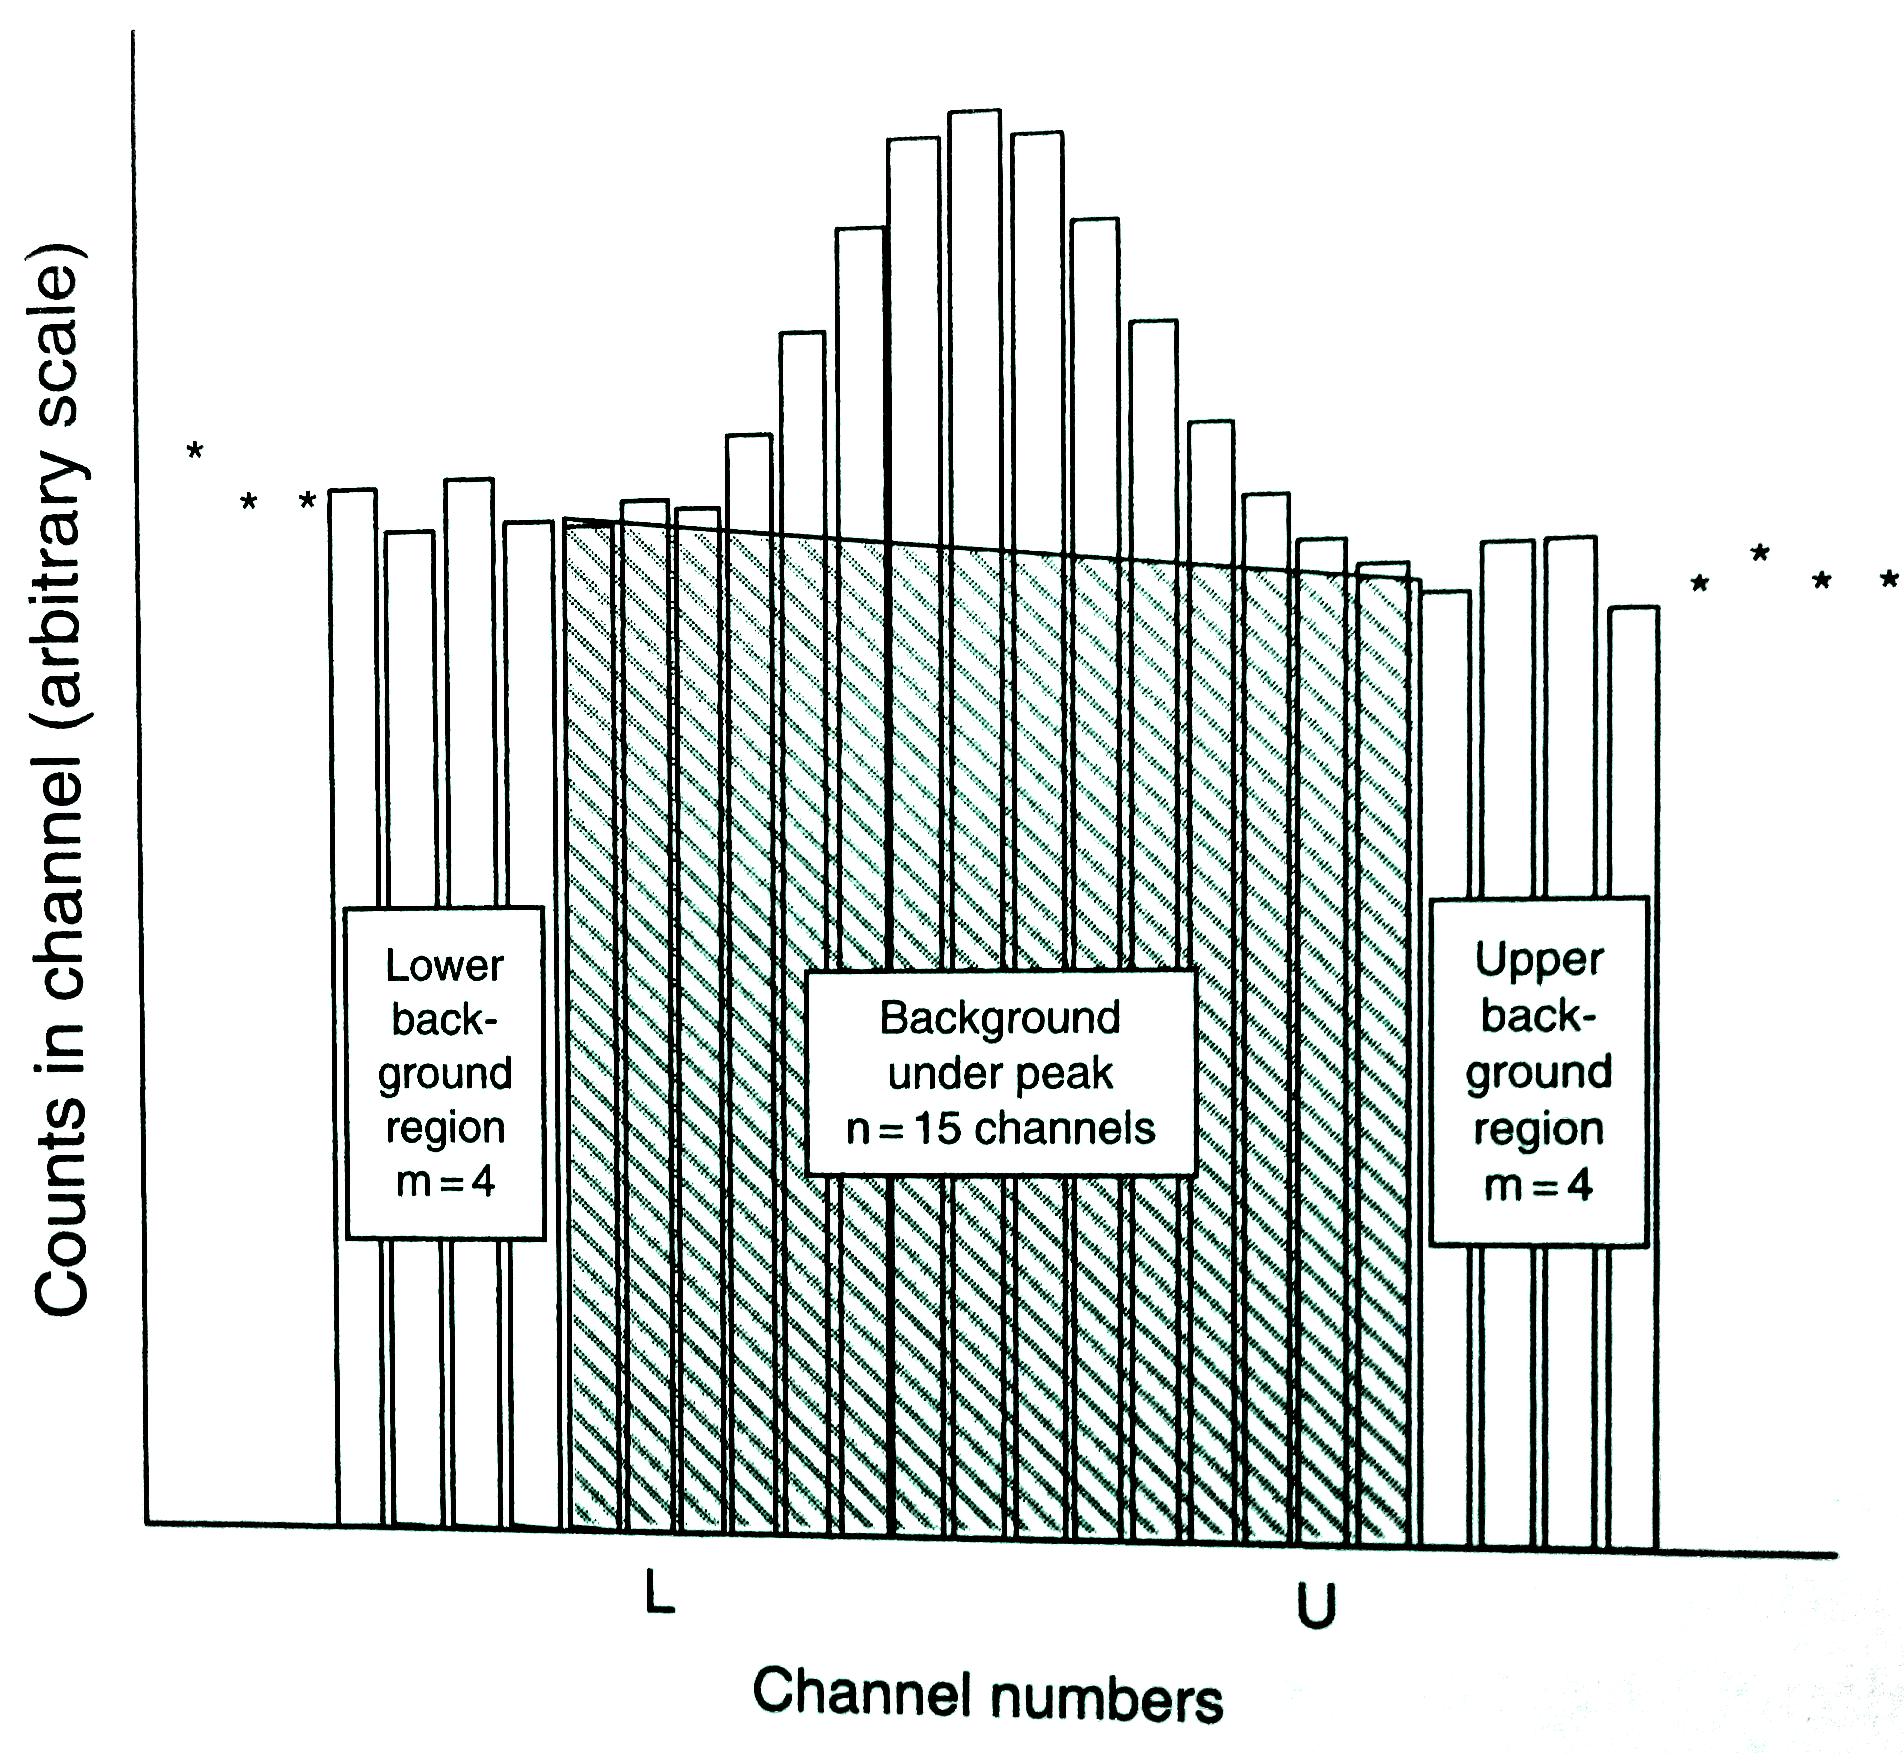
\includegraphics[width=6cm]{images/peak_uncert.png}
\caption{Graphical description of peak area uncertainty estimates.  Reproduced from \cite{Gilmore:1995qr}.}
\label{peak_uncert}
\end{figure}
The uncertainty in the net peak area due purely to counting statistics, $\sigma_{A_c}$ is given by equation \ref{pa_uncert} \cite{Gilmore:1995qr}:
\begin{equation}
    \sigma_{A_c} = \sqrt{A + B(1 + n/2m)}
    \label{pa_uncert}
\end{equation}
Where $A$ is the net peak area, $B$ is the background area under the peak, and $n$ is the number of channels
in the peak region and $m$ is the number of channels in the left and right background regions.  The ratio
$n/m$ is calculated in GammaSpy by searching for the bin locations corresponding to 3 standard deviations
from the mean of the peak.  Since the mean is known via the curve fitting process, it is simple to estimate
$n/m$.  This process is graphically depicted in figure \ref{peak_uncert}. \\

In reality, the model that is fit to the data may not be
the true, correct distribution - the fitted model is merely an estimate.  Each
fitted parameter, $\alpha_i$ carries some uncertainty, $\sigma_{\alpha_i}$.  The estimated parameter values
are assumed to follow a normal distribution as shown in equation \ref{norm_alpha}.
\begin{equation}
\hat \alpha_i = \alpha_i + N(\alpha_i, \sigma_{\alpha_i})
\label{norm_alpha}
\end{equation}
Where $N(\mu, \sigma)$ is the normal distribution.  The goal then is to estimate
$\{\sigma_{\alpha_i} \forall i \}$ and then propagate the model parameter uncertainties to the net area. \\

The uncertainty in each fitted model parameter can be estimated by computing the Hessian of the $\chi^2$ objective
 function at the location of the global minimum.  This approximation is derived by computing the Taylor expansion of the objective function about
 the minimum and ignoring terms higher than order $O^2$.  See \cite{cvonline:2017} and \cite{gavin:2017} for a complete derivation.
The Hessian is related to the covariance matrix by:
\begin{equation}
   \bm C \approx (\bm H)^{-1}
\end{equation}
The diagonal entries of the covariance matrix are estimates for the variance of each model parameter,
$\bm I \bm C = \sigma_{\alpha_1, ... \alpha_n}^2$.
The standard propagation of uncertainty technique is used to estimate the uncertainty in the net
peak area attributed to model uncertainty:
\begin{equation}
    \bm \sigma^2_{A_m} = \bm J_{A_m} \cdot \bm C  \cdot \bm J_{A_m}^T
\end{equation}
Where $\bm J_{A_m}$ is the Jacobian of equation \ref{model_net_area} with respect to the fitted model parameters.  The
vector $\bm J_{A_m}$ is computed by central finite difference. \\

Finally, the total net peak uncertainty is computed via equation \ref{final_uncert}:

\begin{equation}
    \sigma_A = \sqrt{\sigma_{A_c}^2 + \sigma_{A_m}^2}
    \label{final_uncert}
\end{equation}

\subsection{Peak Detection}

The peak detection algorithm is based on the continuous wavelet transform (CWT) in GammaSpy.
The algorithm is fully described by \cite{Du:2006}.
This algorithm was chosen over a derivative search based method because different peaks
in a typical spectrum have slightly different shapes and thus have different first and
second derivatives.  It is difficult, then, to choose a threshold derivative that indicates
the presence of a peak.  Secondly, it is not useful to compute derivatives of the raw
spectrum due to noise; first the spectrum would be smoothed.  This has the consequence of
over smoothing smaller peaks such that the user set derivative detection threshold
is missed.  This results in a plague of false negatives. 
A CWT based approach does not suffer from these deficiencies. \\

The CWT, $C_{a,b}(t)$, of a real valued  signal $s(t)$ is computed by equation \ref{cwt}.

\begin{equation}
    C(a,b) = \frac{1}{\sqrt a}\int_R s(t) \psi_{a,b}(\frac{t-b}{a}) dt
    \label{cwt}
\end{equation}
Where $\psi_{a,b}(t)$ is taken to be the mexican hat wavelet function shown in figure \ref{mhat}.
$R$ is the domain of the signal.

\begin{figure}[!htbp]
\centering
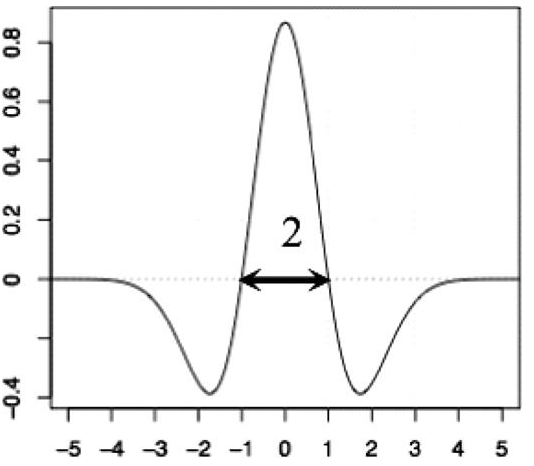
\includegraphics[width=4cm]{images/mexican_hat.png}
\caption{Mexican hat wavelet with $a=1, b=0$. Reproduced from \cite{Du:2006}.}
\label{mhat}
\end{figure}

In the peak detection algorithm, the CWT of the signal is computed for
each entry of a vector, $\bm a$.  The test entries in $\bm a =\{a_0, ... a_N\}$ should
be on the order of the FWHM of the gamma peaks in the spectrum.  The initial
guess for $\bm a$ in GammaSpy is taken to be $[0.2, 0.4, ..., 5.0, 5.2] (KeV)]$.
For each entry in $\bm a$ the CWT is computed.
The wavelet is swept over the signal by modifying the translational parameter, $b \in R$ in small increments on the order of the bin width.
This results in a 2D matrix of $C$ evaluated at many $(a_i, b_i)$ combinations. This can be plotted
as a heat map as shown in figure \ref{cwt_scale}. \\

\begin{figure}[!htbp]
\centering
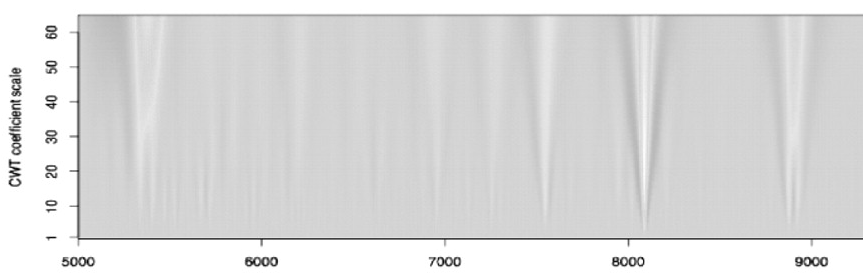
\includegraphics[width=9cm]{images/cwt_scale.png}
\caption{CWT magnitude at different combinations of $a_i, b_i$. Reproduced from \cite{Du:2006}.}
\label{cwt_scale}
\end{figure}

Next, the heat map is inspected row-by-row for local maximum.  This is 1D ridge line search problem
that is relatively easy to solve since the width of the ``bumps'' in each row of the C matrix are known to be
on the order of $\approx 2a_i$ wide.  Once this is done for each row in the $C$ matrix,
peak locations are determined by summing up the magnitude of $C$ column-wise at all identified local maxima.
An example of identified locations and magnitudes of $C$ are shown in figure \ref{cwt_dots}. \\

\begin{figure}[!htbp]
\centering
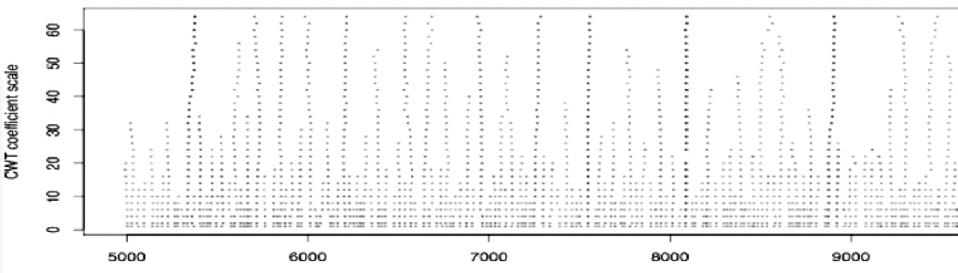
\includegraphics[width=9cm]{images/cwt_dots.png}
\caption{Locations and relative magnitudes of local maxima in $C$. \cite{Du:2006}.}
\label{cwt_dots}
\end{figure}
The relative size of the dots represent the magnitude of the $C$ matrix at the location of an identified local maximum.
Those sums which fall above a user specified threshold (called the signal-to-noise ratio) are marked as peak locations. \\

In the work performed by \cite{Du:2006}, the resilience of the CWT based method to background noise is also demonstrated.
In summary, the CWT can be decomposed into three parts:

\begin{equation}
    C(a,b) = \int P(t)\psi_{a,b}(t) dt + \int B(t) \psi_{a,b}(t) dt + \int C \psi_{a,b} (t)dt
\end{equation}
Where $P$ is the peak-only signal, $B$ is the background, and $C$ is a constant.  It can be shown
that the second and third terms are approximately zero.

%----------------------------------------------------------------------------------------
%	SECTION 3
%----------------------------------------------------------------------------------------

\section{Results}


\subsection{Single Peak}
A comparison between GammaSpy and Cambio for single peak net area calculation was performed
to ascertain if the currently implemented algorithms performed as expected, atleast in
the simple case of a single peak.
The test spectrum used can be downloaded from: \url{https://github.com/wgurecky/GammaSpy/blob/master/examples/data/NORM-H2O.CNF}.
A single peak located at $\approx$ 1120 (KeV) was selected for comparison.  The fitting results from
GammaSpy and Cambio are presented in table \ref{table_1}.

\begin{table}[h]
\begin{center}
\begin{tabular}{|c|c|c|c|c|c|}
\hline 
Code & Energy	&FWHM	&Peak	&Peak	&Peak \\
       & (keV)	&(keV)	&Area	&Uncert.	&Background\\ \hline \hline
 GammaSpy &1119.82	& 1.911	&18293.64 &156.99 & 1285.73 \\
 Cambio &1120.28	& 1.865	&18274.21 &253.61 & N/A \\
\hline
\end{tabular}
\caption{Single peak comparison between GammaSpy and Cambio.}
\end{center}
\label{table_1}
\end{table}

The net area are in agreement with a relative difference of only $0.13\sigma$.  The uncertainty
estimates, however, are significantly different.  It is hypothesized that this difference
is due to the different peak and background functions used in Cambio vs GammaSpy. \\

\begin{figure}[!htbp]
\centering
\begin{minipage}{.55\textwidth}
  \centering
  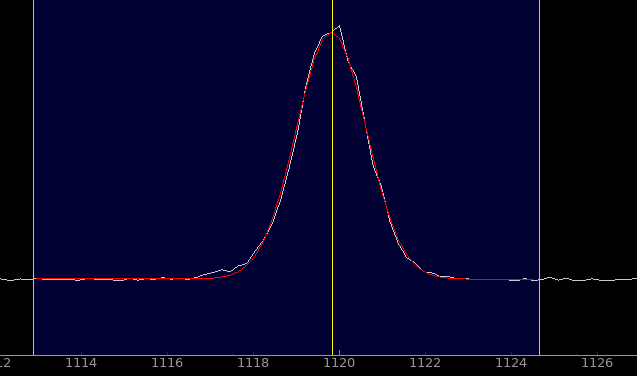
\includegraphics[width=.90\linewidth]{images/gspy_ex.png}
  \captionof{figure}{  GammaSpy fit.}
  \label{fig1}
\end{minipage}%
\begin{minipage}{.55\textwidth}
  \centering
  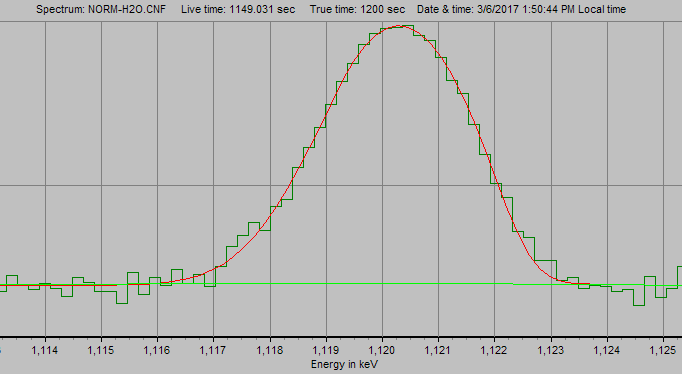
\includegraphics[width=.95\linewidth]{images/cambio_ex.png}
  \captionof{figure}{  Cambio fit.}
  \label{fig2}
\end{minipage}
\end{figure}

It should be noted that Cambio uses a cubic rather than liner background function and
uses a exponentially modified Gaussian function for the peak rather than a pure Gaussian.
These extra complexities (more coefficients to estimate in the model) would result in larger propagated uncertainties in the
net peak area.  This is only a guess since the process by which Cambio estimates uncertainties is unknown.
Since the fitted peak shapes are fundamentally different between the two codes, there is
also a small discrepancy in the predicted FWHM. Additionally, GammaSpy estimates the peak
mean to occur at a slightly smaller energy than Cambio due to the skewed lower tail of the peak
dragging the mean with it. \\

In the future, additional peak trial functions could be added to GammaSpy to achieve better agreement with Cambio.

\subsection{Double Peak}
For the double peak case a comparison with Cambio was not possible since the current
version of Cambio cannot fit multiple nearby peaks.  The results of the following fit
are thus unverified and meant as only a demonstration of GammaSpy's capabilities but
not as measure of validity. \\

\begin{table}[h]
\begin{center}
\begin{tabular}{|c|c|c|c|c|c|}
\hline 
   & Energy	&FWHM	&Peak	&Peak	&Peak \\
       & (keV)	&(keV)	&Area	&Uncert.	&Background\\ \hline \hline
 Peak 1&238.27 & 1.504	&  8477.06 & 158.98 & 7917.03 \\
 peak 2&241.54	& 1.296	& 37884.82  &244.37 & 6653.34 \\
\hline
\end{tabular}
\caption{Double peak fitting results from GammaSpy.}
\end{center}
\label{table_2}
\end{table}

A twin peak located at $\approx$ 240 (KeV) was selected as the target for double peak fitting.
GammaSpy automatically detects that two peaks are nearby and within each other's ROI - this triggers
a double Gaussian fit.  This behaviour can be adjusted if the user wishes to force a single or double
peak fit.  See section \ref{ug} for details.

\begin{figure}[!htbp]
\centering
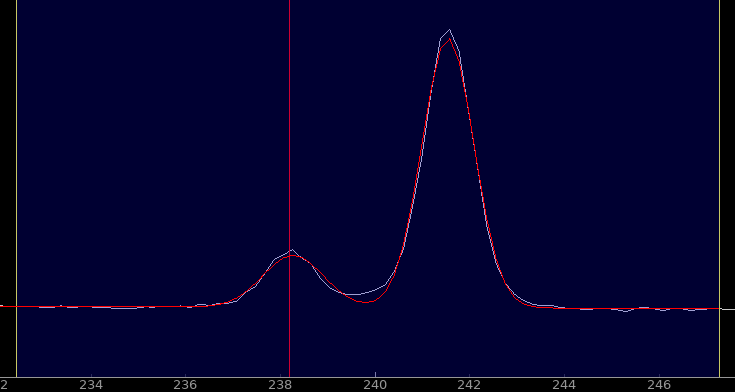
\includegraphics[width=8cm]{images/gspy2_ex.png}
\caption{Double peak fit visualization performed in GammaSpy.}
\label{gui}
\end{figure}

%----------------------------------------------------------------------------------------
%	SECTION 4
%----------------------------------------------------------------------------------------
\pagebreak
\section{Conclusions and Discussion}

The focus of this work was not to develop non-linear curve fitting techniques or improve upon the CWT algorithm,
instead GammaSpy was developed to aggregate useful computational tools in a package
targeted specifically at gamma spectroscopy. The developed package could be useful to those seeking
an alternative to the Cambio or Maestro softwares.  GammaSpy may also be useful as a platform if a curious user
wants to test a new peak fitting or finding algorithm.  The opportunity for
future work is significant.  Additional non-Gaussian peak models could be implemented and the
current linear background assumption could be relaxed.  Additionally, the overall ease of use of the
GUI could be improved.

\pagebreak
\section{Users Guide}
\label{ug}

The main GUI window is presented in figure \ref{gui}.
\begin{figure}[!htbp]
\centering
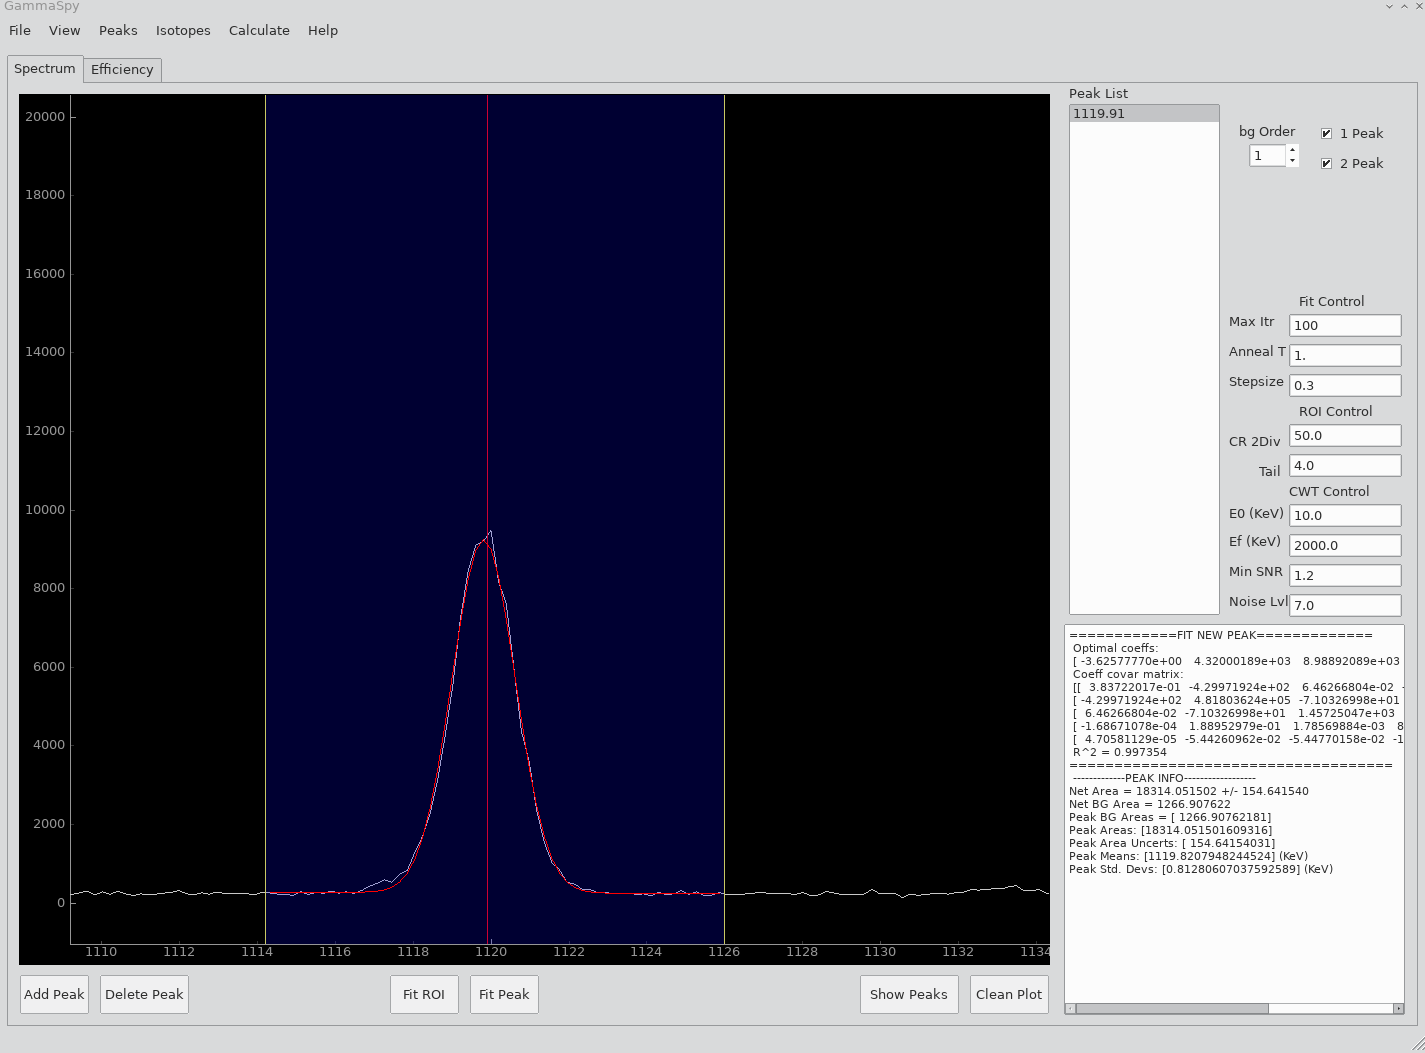
\includegraphics[width=14cm]{images/gui.png}
\caption{Main GUI window.}
\label{gui}
\end{figure}

\subsection*{Basic movement}

\begin{itemize}
    \item \textbf{Middle Mouse + drag}:  Spectrum pan.
    \item \textbf{Left Mouse + drag}:  Pan or move ROI marker depending on context.
    \item \textbf{Right Mouse + drag}:  Spectrum zoom.
    \item \textbf{Right Mouse}: Open graphical option menu.
\end{itemize}
To reset the view, \textbf{Right Click} the plot area and select \textbf{View All}.

After peaks have been added to the peak list (see below), the selected peak can be
cycled through by pressing the keyboard hotkeys:
\begin{itemize}
    \item \textbf{j}: select next peak in list
    \item \textbf{k}: select previous peak in list
\end{itemize}

\subsection*{Adding Peaks}

\subsubsection*{\ \ Manual Peak Add}
The peak marker is positioned by using the keyboard shortcut \textbf{ctrl + a}.
After the peak marker is positioned where desired, click the \textbf{Add Peak} button.

\subsubsection*{\ \ Automatic Peak Add}
Peaks can automatically be found by selecting the auto-peaks option form the
\textbf{Peaks $\rightarrow$ Auto Peaks} menu item.  The peak list will be automatically updated
with the peaks found by the CWT algorithm.

\subsubsection*{\ \ Delete Peaks}
Select a peak in the peak list to the right of the spectrum plot.  Then click the
\textbf{delete peak} button or use the keyboard shortcut \textbf{ctrl + d}.

\subsection*{Marking the ROI}
\begin{figure}[!htbp]
\centering
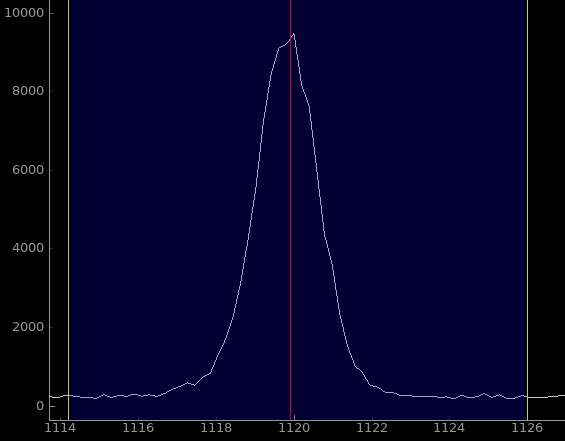
\includegraphics[width=6cm]{images/roi_ex.png}
\caption{ROI zone markers shown, with ROI overlaying the spectrum plot.}
\label{roi_ex}
\end{figure}

\subsubsection*{\ \ Manual ROI}
First, select a peak from the peak list.  An ROI zone marker will appear in the spectrum plot window.
Drag the left and right bounds of the ROI marker as desired using \textbf{Left Mouse + drag}.

\subsubsection*{\ \ Automatic ROI}
The ROI can also be automatically estimated by first selecting a peak from the peak list
and then clicking the \textbf{Fit ROI} button.

\subsection*{Fit Peaks}

Select a peak from the list.  Click the \textbf{Fit Peak} button.  The parameters to
the fitting routine can be adjusted by editing the settings on the right of the spectrum plot window.
After fitting, the model function will be displayed as a red line overlaying the original data.
Peak fitting info will be provided in the output window on the right hand side of the screen.
\begin{figure}[!htbp]
\centering
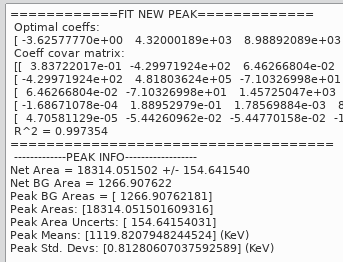
\includegraphics[width=6cm]{images/peak_out_ex.png}
\caption{Output peak fitting info.}
\label{output}
\end{figure}

\subsubsection*{Force Single or Double Gaussian Fit}
The check boxes on the right of the GammaSpy window can be toggled such that only
a single or double Gaussian is considered when fitting.  Both check boxes are
enabled by default so that both a single and double Gaussian fit is considered.
If two peaks are located inside each other's ROI, then a double Gaussian fit will
automatically be selected.

\subsection*{Saving Peak Info}
To save all fitted peak info, choose the \textbf{Peaks $\rightarrow$ Peak Report} Menu option.
Specify the filename of the desired output file.  This output file will be in plain text.

\pagebreak
%----------------------------------------------------------------------------------------
%	BIBLIOGRAPHY
%----------------------------------------------------------------------------------------

\bibliographystyle{apalike}

\bibliography{sample}

%----------------------------------------------------------------------------------------


\end{document}
